\documentclass[preview]{standalone}
\usepackage{pgfplots}
\begin{document}

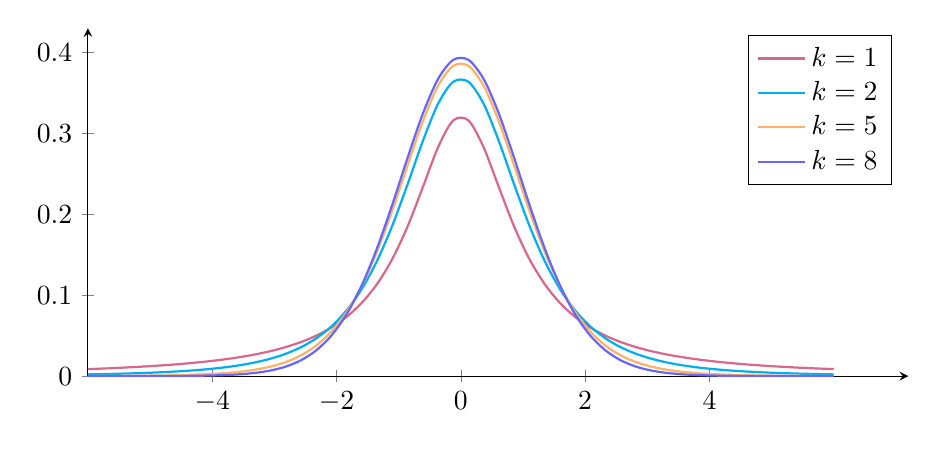
\begin{tikzpicture}[
    declare function={gamma(\z)=
    2.506628274631*sqrt(1/\z)+ 0.20888568*(1/\z)^(1.5)+ 0.00870357*(1/\z)^(2.5)- (174.2106599*(1/\z)^(3.5))/25920- (715.6423511*(1/\z)^(4.5))/1244160)*exp((-ln(1/\z)-1)*\z;},
    declare function={student(\x,\n)= gamma((\n+1)/2.)/(sqrt(\n*pi) *gamma(\n/2.)) *((1+(\x*\x)/\n)^(-(\n+1)/2.));}
]

\begin{axis}[
  width=12cm,height=6cm,
    axis lines=left,
    enlargelimits=upper,
    samples=50,
    xtick={-4,-2,...,4},
    legend entries={$k=1$,$k=2$,$k=5$,$k=8$}
]
\pgfplotsinvokeforeach{1}{
    \addplot [thick, smooth, domain=-6:6, purple!60] {student(x,#1)};
}
\pgfplotsinvokeforeach{3}{
  \addplot [thick, smooth, domain=-6:6, cyan] {student(x,#1)};
}
\pgfplotsinvokeforeach{8}{
    \addplot [thick, smooth, domain=-6:6, orange!60] {student(x,#1)};
}
\pgfplotsinvokeforeach{20}{
    \addplot [thick, smooth, domain=-6:6, blue!60] {student(x,#1)};
}
\end{axis}
\end{tikzpicture}
\end{document}